\section*{Appendix}

\subsection*{Site split formulation}
We begin by introducing ``site splits.''
We use site splits to formalize the notion that a given site pattern is equally probable to its complement under the binary symmetric model.
This is a standard step in the description of the Hadamard transform (Section 8.6 of \citet{Semple2003-em}), although our approach is complicated slightly by the inclusion of ancestral states.

Since we have a finite character alphabet, for a given column $i$ there are a finite number of possible assignments of characters to tips $\alignmentColumn_i$ or internal nodes $\ancestralStateColumn_i$.
For the binary symmetric model, the alphabet $\alphabet$ is $\{0,1\}$.
Take the tip labels of $\tau$ to be $\{1,\ldots,\nSiteRows\}$.
For likelihood calculation under the binary symmetric model, we describe a given $\alignmentColumn_i$ as a subset of indices $\siteSplit\subseteq\siteSplitSet:=\{1,\ldots,\nSiteRows-1\}$, commonly called a ``site split.''
Define the complement of $\alignmentColumn$ as $\overline{\alignmentColumn}$, and let $\alignmentColumn_{i,k}$ be the label of the $k$th tip in the $i$th alignment column.
We define the site split $\siteSplit$ for a $\alignmentColumn_i$ as the set of tips labeled with $1$ in $\alignmentColumn_i$ if the $\nSiteRows$th tip is not labeled with $1$, and as the set of tips labeled with $1$ in $\overline{\alignmentColumn}_i$ if the $\nSiteRows$th tip is labeled with $1$.
Taking such a complement simplifies but does not change the result of likelihood computation because the probability of observing a particular collection of binary characters is equivalent to the probability of its complement under the binary symmetric model.

For a fixed topology $\tau$, we define an ordered set of internal node labels $\{1,\ldots,\nAncestralStateRows\}$ for $\ancestralStateColumn_i$ and similarly use a subset of characters $\ancestralSplit\subseteq\ancestralSplitSet:=\{1,\ldots,\nAncestralStateRows\}$ to describe a realization $\ancestralStateColumn_i$.
In this case we cannot use the same complement trick as before: the probability of observing an ancestral state split conditional on a site split is not invariant to taking its complement.
We thus define an ``ancestral state split'' $\ancestralSplit$ for an internal node $\ancestralStateColumn_i$ to be the set of internal nodes labeled with $1$ if the $\nSiteRows$th tip is not labeled with $1$, and as the set of internal nodes labeled with $1$ in $\overline{\ancestralStateColumn}_i$ if the $\nSiteRows$th tip is labeled with $1$.
We emphasize that the ancestral state split complementing procedure depends on tip states, not ancestral states: both site splits and ancestral state splits are defined by whether the $\nSiteRows$th element of $\alignmentColumn_i$ is labeled as $1$.

We enumerate the site splits $\siteSplit_j$ of which there are $\nSiteSplits=|\mathcal{P}(\siteSplitSet)|$ in total where $\mathcal{P}$ denotes the power set.
Similarly we enumerate ancestral state splits $\ancestralSplit_k$ of which there are $\nAncestralSplits=|\mathcal{P}(\ancestralSplitSet)|$ in total.

We first fix notation.
\begin{definition}
Let the mapping from site patterns to site splits
\[
\patternToSplit:\alphabet^\nSiteRows\rightarrow\mathcal{P}(\siteSplitSet)
\]
be
\[
\patternToSplit(\alignmentColumn) =
\left\{
    \begin{array}{ll}
        \{i'\in\{1,\ldots,\nSiteRows-1\}: \alignmentColumn_{i,i'}=1\}  & \mbox{if } \alignmentColumn_{i,\nSiteRows}=0,\\
        \{i'\in\{1,\ldots,\nSiteRows-1\}: \overline{\alignmentColumn}_{i,i'}=1\}  & \mbox{if } \alignmentColumn_{i,\nSiteRows}=1,
    \end{array}
\right.
\]
and the mapping from ancestral states and tip states to ancestral state splits
\[
\ancestralToSplit:\alphabet^\nSiteRows\times\alphabet^\nAncestralStateRows\rightarrow\mathcal{P}(\ancestralSplitSet)
\]
be
\[
\ancestralToSplit(\alignmentColumn, \ancestralStateColumn) =
\left\{
    \begin{array}{ll}
        \{i'\in\{1,\ldots,\nAncestralStateRows\}: \ancestralStateColumn_{i,i'}=1\}  & \mbox{if } \alignmentColumn_{i,\nSiteRows}=0,\\
        \{i'\in\{1,\ldots,\nAncestralStateRows\}: \overline{\ancestralStateColumn}_{i,i'}=1\}  & \mbox{if } \alignmentColumn_{i,\nSiteRows}=1.
    \end{array}
\right.
\]
Then, given a site pattern--valued random variable $\alignmentColumnRV$ and an ancestral state--valued random variable $\ancestralStateColumnRV$, define the random variables
\[
\siteSplitRV := \patternToSplit(\alignmentColumnRV)
\]
and
\[
\ancestralSplitRV := \ancestralToSplit(\alignmentColumnRV, \ancestralStateColumnRV).
\]
\end{definition}
The mapping $\patternToSplit$ operates by returning the tips labeled as $1$ in a site pattern to obtain a site split in $\mathcal{P}(\siteSplitSet)$ if the set of tips labeled $1$ is not in $\mathcal{P}(\siteSplitSet)$.
The mapping $\ancestralToSplit$ is defined by whether the tip states have their complements taken or not: if the set of tips labeled $1$ in $\alignmentColumn$ is in $\mathcal{P}(\siteSplitSet)$, $\ancestralToSplit(\alignmentColumn, \ancestralStateColumn)$ is the set of tips labeled $1$ in $\ancestralStateColumn$; otherwise, the set of tips labeled $1$ in $\overline{\alignmentColumn}$ necessarily is in $\mathcal{P}(\siteSplitSet)$ and so $\ancestralToSplit(\alignmentColumn, \ancestralStateColumn)$ is $\overline{\ancestralStateColumn}$.

For the $i$th factor of \eqref{eq:full_likelihood}, we decompose the likelihood into its marginal and conditional components as
\[
\Pr(\alignmentColumnRV=\alignmentColumn_i, \ancestralStateColumnRV=\ancestralStateColumn_i \mid \tau, t) = \Pr(\alignmentColumnRV=\alignmentColumn_i \mid \tau, t) \cdot \Pr(\ancestralStateColumnRV=\ancestralStateColumn_i \mid \alignmentColumnRV=\alignmentColumn_i, \tau, t).
\]
As a consequence of assuming a binary symmetric model, for some $\siteSplit_j\in\mathcal{P}(\siteSplitSet)$ the mapping $\patternToSplit(\alignmentColumn_i)$ has the property
\begin{align*}
    \Pr(\siteSplitRV=\siteSplit_j \mid \tau, t) &= \Pr(\siteSplitRV=\patternToSplit(\alignmentColumn_i) \mid \tau, t)\\
    &= \Pr(\alignmentColumnRV=\alignmentColumn_i \cup \overline{\alignmentColumnRV}=\alignmentColumn_i \mid \tau, t)\\
    &= \Pr(\alignmentColumnRV=\alignmentColumn_i \mid \tau, t) + \Pr(\overline{\alignmentColumnRV}=\alignmentColumn_i \mid \tau, t)\\
    &= 2\cdot\Pr(\alignmentColumnRV=\alignmentColumn_i \mid \tau, t)
\end{align*}
where $\overline{Y}$ is the complement of the site pattern--valued random variable $Y$ and has the same distribution as $Y$.
Note
\begin{align*}
    \Pr(\ancestralStateColumnRV=\ancestralStateColumn_i \mid \alignmentColumnRV=\alignmentColumn_i, \tau, t) &= \Pr(\ancestralSplitRV=\ancestralToSplit(\alignmentColumn_i, \ancestralStateColumn_i) \mid \siteSplitRV=\patternToSplit(\alignmentColumn_i), \tau, t).
\end{align*}
Thus given $(\tau, t)$, there exist sets $\ancestralSplitPartition_1(\tau, t),\ldots,\ancestralSplitPartition_\nSiteSplits(\tau, t)$ such that $\xi_j\in\ancestralSplitPartition_j(\tau, t)$ satisfies
\begin{align*}
\max_{\ancestralSplit_k\in\mathcal{P}(\ancestralSplitSet)} \ \Pr(\ancestralSplitRV=\ancestralSplit_k \mid \siteSplitRV=\siteSplit_j, \tau, t) &= \Pr(\ancestralSplitRV = \xi_j \mid \siteSplitRV=\siteSplit_j, \tau, t).
\end{align*}
In other words, for the $j$th site split, $\ancestralSplitPartition_j(\tau, t)\subseteq\mathcal{P}(\ancestralSplitSet)$ is the set of most likely ancestral state splits for that particular site split, topology and set of branch lengths, i.e., $\ancestralSplitPartition_j(\tau, t)$ is a set of sets of most likely internal node labels.
Here, $\xi_j$ is one of possibly many equiprobable ancestral state splits in $\ancestralSplitPartition_j(\tau, t)$.
For each $\alignmentColumn_i$, $\ancestralToSplit(\alignmentColumn_i, \cdot)$ is surjective as it can map values from $\alphabet^\nAncestralStateRows$ to all elements in $\mathcal{P}(\ancestralSplitSet)$.
This can be seen by using the definition of $\ancestralToSplit(\alignmentColumn_i, \cdot)$ and assuming $\alignmentColumn_{i,\nSiteRows}=0$, where in this case each of the $2^\nAncestralStateRows$ values of $\ancestralStateColumn$ correspond to each of the $2^\nAncestralStateRows$ elements of $\mathcal{P}(\{1,\ldots,\nAncestralStateRows\})$.
The same can be done for the case of $\alignmentColumn_{i,\nSiteRows}=1$, implying $\ancestralToSplit(\alignmentColumn_i, \cdot)$ is surjective.
From this we have
\begin{align*}
    \max_{\ancestralStateColumn_i} \ \Pr(\ancestralStateColumnRV=\ancestralStateColumn_i \mid \alignmentColumnRV=\alignmentColumn_i, \tau, t) &= \max_{\ancestralStateColumn_i} \ \Pr(\ancestralSplitRV=\ancestralToSplit(\alignmentColumn_i, \ancestralStateColumn_i) \mid \siteSplitRV=\patternToSplit(\alignmentColumn_i), \tau, t)\\
    &= \max_{\ancestralSplit_k\in\mathcal{P}(\ancestralSplitSet)} \ \Pr(\ancestralSplitRV=\ancestralSplit_k \mid \siteSplitRV=\siteSplit_j, \tau, t)\\
    &= \Pr(\ancestralSplitRV = \xi_j \mid \siteSplitRV=\siteSplit_j, \tau, t)
\end{align*}
for some $j$.
Thus, each term in the likelihood can be collapsed into terms relating only to site splits and ancestral state splits, indexed by $j$, as opposed to individual observations, indexed by $i$.

\subsection*{Example}
We follow with an example computing these probabilities and likelihoods.
Consider the fixed, binary four-taxon tree $\tau_1$ in Fig.~\ref{fig:farris-fels-top}a.
The set of all possible character assignments is
\begin{align*}
\mathcal{P}(\{1,2,3,4\}) &= \{\emptyset, \{1,2,3,4\}, \{1\}, \{2,3,4\}, \{2\}, \{1,3,4\}, \{3\}, \{1,2,4\}, \\
                         &\qquad \{1,2\}, \{3,4\}, \{1,3\}, \{2,4\}, \{2,3\}, \{1,4\}, \{1,2,3\}, \{1,4\}\}
\end{align*}
where each set indicates the tips assigned the character $1$.
For example, $\emptyset$ is the labeling $0000$ and $\{1,3,4\}$ is the labeling $1011$.
Symmetry allows us to group adjacent pairs in $\mathcal{P}(\{1,2,3,4\})$ into equiprobable splits, letting $\siteSplitSet=\{1,2,3\}$.
The unique site splits, collapsing complements, are
\begin{align*}
    \mathcal{P}(\siteSplitSet) &= \{\emptyset, \{1\}, \{2\}, \{3\}, \{1,2\}, \{1,3\}, \{2,3\}, \{1,2,3\}\} \\
& := \{\siteSplit_1, \ldots, \siteSplit_8\}.
\end{align*}
Since we identify character complements, we do not consider the additional splits
\begin{equation*}
\begin{split}
& \mathcal{P}(\{1,2,3,4\}) \setminus \mathcal{P}(\siteSplitSet) = \\
&\qquad \{\{1,2,3,4\}, \{2,3,4\}, \{1,3,4\}, \{1,2,4\}, \{3,4\}, \{2,4\}, \{1,4\}, \{4\}\},
\end{split}
\end{equation*}
the symmetry of the binary character model allowing us to focus only on the elements of $\mathcal{P}(\siteSplitSet)$.
This tree has two internal nodes with $\ancestralSplitSet=\{1,2\}$ and unique ancestral state splits
\[
\mathcal{P}(\ancestralSplitSet) = \{\emptyset, \{1\}, \{2\}, \{1,2\}\}.
\]
Internal node $1$ is the node connected to leaves $1$ and $3$ while internal node $2$ is connected to leaves $2$ and $4$.
The mapping from characters to splits in this case depends on the characters at the tips and the ancestral states.
For example, we take both $\patternToSplit(0000)=\emptyset$ and $\patternToSplit(1111)=\emptyset$.
Similarly, we have $\ancestralToSplit(0000, 00) = \emptyset$ and $\ancestralToSplit(1111, 11)=\emptyset$, needing to take the complement of all the characters present on the tree to identify splits.
We cannot identify complements for ancestral states in the same way as tip states since, for $\siteSplit\in\mathcal{P}(\siteSplitSet)$,
\[
\Pr(\ancestralSplitRV=\emptyset \mid \siteSplitRV=\siteSplit, \tau, t)\neq \Pr(\ancestralSplitRV=\{1,2\} \mid \siteSplitRV=\siteSplit, \tau, t)
\]
in general.

For each site split $\siteSplit\in\mathcal{P}(\siteSplitSet)$, we maximize the likelihood over all $\ancestralSplit\in\mathcal{P}(\ancestralSplitSet)$.
A maximum occurs at one of possibly several ancestral state splits in $\mathcal{P}(\ancestralSplitSet)$, defined via $\ancestralSplitPartition_j(\tau, t)$ for the $j$th site split.
As a simple example, say all branch lengths correspond to a probability $p$ ($< 1/2$) of changing character along that branch, with $t=\{p,p,p,p,p\}$.
The probabilities of observing ancestral state splits for $\siteSplit_1=\emptyset$ are
\[
\Pr(\ancestralSplitRV=\emptyset \mid \siteSplitRV=\emptyset, \tau, t) =
(1-p)^5,
\]
\[
\Pr(\ancestralSplitRV=\{1\} \mid \siteSplitRV=\emptyset, \tau, t) =
\Pr(\ancestralSplitRV=\{2\} \mid \siteSplitRV=\emptyset, \tau, t) =
p^3(1-p)^2,
\]
\[
\Pr(\ancestralSplitRV=\{1,2\} \mid \siteSplitRV=\emptyset, \tau, t) =
p^4(1-p).
\]
The set of most likely ancestral states contains a single element, here $\ancestralSplitPartition_1(\tau, t)=\{\emptyset\}$.
Then, taking $\xi_1\in\ancestralSplitPartition_1(\tau, t)$ we have
\[
\Pr(\ancestralSplitRV=\xi_1 \mid \siteSplitRV=\emptyset, \tau, t) =
\Pr(\ancestralSplitRV=\emptyset \mid \siteSplitRV=\emptyset, \tau, t) =
(1-p)^5.
\]
For $\siteSplit_5=\{1,2\}$ we have
\[
\Pr(\ancestralSplitRV=\emptyset \mid \siteSplitRV=\{1,2\}, \tau, t) =
\Pr(\ancestralSplitRV=\{1,2\} \mid \siteSplitRV=\{1,2\}, \tau, t) =
p^2(1-p)^3,
\]
\[
\Pr(\ancestralSplitRV=\{1\} \mid \siteSplitRV=\{1,2\}, \tau, t) =
\Pr(\ancestralSplitRV=\{2\} \mid \siteSplitRV=\{1,2\}, \tau, t) =
p^3(1-p)^2.
\]
Here, the set of most likely ancestral states is $\ancestralSplitPartition_5(\tau, t)=\{\emptyset,\{1,2\}\}$, and, for $\xi_5\in\ancestralSplitPartition_5(\tau, t)$,
\[
\Pr(\ancestralSplitRV=\xi_5 \mid \siteSplitRV=\{1,2\}, \tau, t) =
p^2(1-p)^3.
\]

\subsection*{Site split likelihood}

The likelihood in \eqref{eq:profile_likelihood} can be written as
\begin{align}
L_\nCols'(\tau, t; \fullAlignment) &= \max_{\fullAncestralStates} \ L_\nCols(\tau, t; \fullAlignment, \fullAncestralStates) \nonumber \\
                             &= \prod_{i=1}^{\nCols} \ \max_{\ancestralStateColumn_i} \ \Pr(\alignmentColumnRV=\alignmentColumn_i, \ancestralStateColumnRV=\ancestralStateColumn_i \mid \tau, t) \nonumber \\
                             &\propto \prod_{i=1}^{\nCols} \ \max_{\ancestralStateColumn_i} \ \Pr(\siteSplitRV=\patternToSplit(\alignmentColumn_i) \mid \tau, t) \cdot \Pr(\ancestralSplitRV=\ancestralToSplit(\alignmentColumn_i, \ancestralStateColumn_i) \mid \siteSplitRV=\patternToSplit(\alignmentColumn_i), \tau, t) \nonumber \\
                             &= \prod_{i=1}^{\nCols} \ \Pr(\siteSplitRV=\patternToSplit(\alignmentColumn_i) \mid \tau, t) \cdot \max_{\ancestralStateColumn_i} \Pr(\ancestralSplitRV=\ancestralToSplit(\alignmentColumn_i, \ancestralStateColumn_i) \mid \siteSplitRV=\patternToSplit(\alignmentColumn_i), \tau, t) \nonumber \\
                             &= \prod_{j=1}^{\nSiteSplits} \ \left[\Pr(\siteSplitRV=\siteSplit_j \mid \tau, t)\cdot \Pr(\ancestralSplitRV=\xi_j \mid \siteSplitRV=\siteSplit_j, \tau, t)\right] ^{\nCols_j(\fullAlignment)} \label{eq:site_pattern_likelihood}
\end{align}
for $\siteSplit_j\in\mathcal{P}(\siteSplitSet)$ and some $\xi_j\in\ancestralSplitPartition_j(\tau, t)$ with $1 \le j \le q$ where $\nCols_j(\fullAlignment)$ is the number of columns in $\fullAlignment$ that project to site split $\siteSplit_j$.

Let
\[
L_\nCols''(\tau, t; \fullAlignment) = \prod_{j=1}^{\nSiteSplits} \ \left[\Pr(\siteSplitRV=\siteSplit_j \mid \tau, t) \cdot \Pr(\ancestralSplitRV=\xi_j \mid \siteSplitRV=\siteSplit_j, \tau, t)\right] ^{\nCols_j(\fullAlignment)}
\]
be the final product in \eqref{eq:site_pattern_likelihood}.
Assume $\nCols$ observations are generated from a model with parameters $(\tau^*, t^*)$.
We have
\begin{equation*}
\begin{split}
&    \frac{1}{\nCols} \log L_\nCols''(\tau, t; \fullAlignment) \\
&\qquad = \sum_{j=1}^\nSiteSplits \frac{\nCols_j(\fullAlignment)}{\nCols}\cdot  \log \Pr(\siteSplitRV=\siteSplit_j, \ancestralSplitRV=\xi_j \mid \tau, t) \\
&\qquad = \sum_{j=1}^\nSiteSplits \frac{\nCols_j(\fullAlignment)}{\nCols}\cdot [\log \Pr(\siteSplitRV=\siteSplit_j \mid \tau, t) +
            \log \Pr(\ancestralSplitRV=\xi_j \mid \siteSplitRV=\siteSplit_j , \tau, t)]
\end{split}
\end{equation*}
so that, in the $\nCols\rightarrow\infty$ limit,
\begin{equation}
\begin{split}
&    \frac{1}{\nCols} \log L_\nCols''(\tau, t; \fullAlignment) \\
&\qquad \rightarrow \sum_{j=1}^\nSiteSplits \Pr(\siteSplitRV=\siteSplit_j \mid \tau^*, t^*) \cdot [\log \Pr(\siteSplitRV=\siteSplit_j \mid \tau, t) + \log \Pr(\ancestralSplitRV=\xi_j \mid \siteSplitRV=\siteSplit_j , \tau, t)]. \label{eq:site_pattern_profile_likelihood_mean}
\end{split}
\end{equation}
Define the marginal log-likelihood
\[
\shannonDivergence_{\tau^*,t^*}(\tau,t) = \sum_{j=1}^\nSiteSplits \Pr(\siteSplitRV=\siteSplit_j \mid \tau^*, t^*)\cdot\log \Pr(\siteSplitRV=\siteSplit_j \mid \tau, t)
\]
and the conditional log-likelihood
\[
\ell^C_{\tau^*,t^*}(\tau, t; \boldsymbol\xi) = \sum_{j=1}^\nSiteSplits \Pr(\siteSplitRV=\siteSplit_j \mid \tau^*, t^*)\cdot\log \Pr(\ancestralSplitRV=\xi_j \mid \siteSplitRV = \siteSplit_j, \tau, t)
\]
with $\boldsymbol\xi = [\xi_j]_{j=1}^\nSiteSplits$ so that \eqref{eq:site_pattern_profile_likelihood_mean} is
\begin{equation}
    \label{eq:log_likelihood_simplified}
    \ell_{\tau^*,t^*}(\tau, t; \boldsymbol\xi) = \shannonDivergence_{\tau^*,t^*}(\tau,t) + \ell^C_{\tau^*,t^*}(\tau, t; \boldsymbol\xi).
\end{equation}

\subsection*{Hadamard representation}

We state the Hadamard representation of site split generating probabilities---that is, probabilities of obtaining particular site splits given a tree---following Section 8.6 of \citet{Semple2003-em}.
For each edge $e$ define the edge ``fidelity'' for that edge as
\[
\theta(e) = 1-2p(e)
\]
where $p(e)$ is the probability of a character change along edge $e$.
For an even-sized subset of $Y\subseteq\mathcal{S}$, let the path set $P(Y)$ be the set of edges in the path connecting both elements of $Y$.
For $n$ taxa, the probability of observing site split $A\in\mathcal{P}(\siteSplitSet)$ is
\begin{equation}
\label{eq:hadamard_probability}
p_A = \frac{1}{2^{n-1}} \ \sum_{Y \subseteq \mathcal{S} : |Y| \equiv 0 (\mathrm{mod} \ 2)} \ \left[(-1)^{|Y \cap A|} \ \prod_{e\in P(Y)} \ \theta(e) \right].
\end{equation}
By convention, we set $P(\emptyset)=\emptyset$ and $\prod_{e\in\emptyset} \ \theta(e) = 1$.
For notational convenience, let
\[
p_{\siteSplit_j} := \Pr(\siteSplitRV=\siteSplit_j \mid \tau_1,t),
\]
for any site split $\siteSplit_j$.
Table~\ref{tab:gen-sitepatprob} contains calculations of site split probabilities for the trees in Fig.~\ref{fig:farris-fels-top}.

\begin{table}[ht]
\centering
\begin{tabular}{|l|l|l|}
    \multicolumn{3}{c}{InvFels tree $\tau=\tau^*$, $t^*=\{x^*,y^*,x^*,y^*,y^*\}$}\\
    \hline
$\siteSplit_j$  & $p_{\siteSplit_j}$ &$8\cdot\Pr(\siteSplitRV=\siteSplit_j \mid \tau,t)$\\
    \hline
    $\emptyset$ & $p_{\emptyset}$   &$1+(x^*)^2+(y^*)^2+4x^*(y^*)^2+(x^*)^2(y^*)^2$\\
    $\{1\}$     & $p_{1}$           &$1-(x^*)^2+(y^*)^2-(x^*)^2(y^*)^2$\\
    $\{2\}$     & $p_{2}$           &$1+(x^*)^2-(y^*)^2-(x^*)^2(y^*)^2$\\
    $\{3\}$     & $p_{3}$           &$1-(x^*)^2+(y^*)^2-(x^*)^2(y^*)^2$\\
    $\{1,2,3\}$ & $p_{123}$         &$1+(x^*)^2-(y^*)^2-(x^*)^2(y^*)^2$\\
    $\{1,2\}$   & $p_{12}$          &$1-(x^*)^2-(y^*)^2+(x^*)^2(y^*)^2$\\
    $\{2,3\}$   & $p_{23}$          &$1-(x^*)^2-(y^*)^2+(x^*)^2(y^*)^2$\\
    $\{1,3\}$   & $p_{13}$          &$1+(x^*)^2+(y^*)^2-4x^*(y^*)^2+(x^*)^2(y^*)^2$\\
    \hline
    \multicolumn{3}{c}{InvFels tree $\tau=\tau_1$, $t=\{x_1,y_1,x_2,y_2,w\}$}\\
    \hline
$\siteSplit_j$  & $p_{\siteSplit_j}$ &$8\cdot\Pr(\siteSplitRV=\siteSplit_j \mid \tau,t)$\\
    \hline
    $\emptyset$ & $p_{\emptyset}$   &$1 + x_1x_2 +  y_1y_2 +  w[  x_1 + x_2][  y_1 + y_2] + x_1y_1x_2y_2$\\
    $\{1\}$     & $p_{1}$           &$1 - x_1x_2 +  y_1y_2 +  w[- x_1 + x_2][  y_1 + y_2] - x_1y_1x_2y_2$\\
    $\{2\}$     & $p_{2}$           &$1 + x_1x_2 -  y_1y_2 +  w[  x_1 + x_2][- y_1 + y_2] - x_1y_1x_2y_2$\\
    $\{3\}$     & $p_{3}$           &$1 - x_1x_2 +  y_1y_2 +  w[  x_1 - x_2][  y_1 + y_2] - x_1y_1x_2y_2$\\
    $\{1,2,3\}$ & $p_{123}$         &$1 + x_1x_2 -  y_1y_2 +  w[  x_1 + x_2][  y_1 - y_2] - x_1y_1x_2y_2$\\
    $\{1,2\}$   & $p_{12}$          &$1 - x_1x_2 -  y_1y_2 +  w[- x_1 + x_2][- y_1 + y_2] + x_1y_1x_2y_2$\\
    $\{2,3\}$   & $p_{23}$          &$1 - x_1x_2 -  y_1y_2 +  w[  x_1 - x_2][- y_1 + y_2] + x_1y_1x_2y_2$\\
    $\{1,3\}$   & $p_{13}$          &$1 + x_1x_2 +  y_1y_2 +  w[- x_1 - x_2][  y_1 + y_2] + x_1y_1x_2y_2$\\
    \hline
    \multicolumn{3}{c}{Felsenstein tree $\tau=\tau_2$, $t=\{x_1,y_1,x_2,y_2,w\}$}\\
    \hline
$\siteSplit_j$  & $p_{\siteSplit_j}$ &$8\cdot\Pr(\siteSplitRV=\siteSplit_j \mid \tau,t)$\\
    \hline
    $\emptyset$ & $p_{\emptyset}$   &$1 + x_1y_1 +  x_2y_2 +  w[  x_1 + y_1][  x_2 + y_2] + x_1y_1x_2y_2$\\
    $\{1\}$     & $p_{1}$           &$1 - x_1y_1 +  x_2y_2 +  w[ -x_1 + y_1][  x_2 + y_2] - x_1y_1x_2y_2$\\
    $\{2\}$     & $p_{2}$           &$1 - x_1y_1 +  x_2y_2 +  w[  x_1 - y_1][  x_2 + y_2] - x_1y_1x_2y_2$\\
    $\{3\}$     & $p_{3}$           &$1 + x_1y_1 -  x_2y_2 +  w[  x_1 + y_1][ -x_2 + y_2] - x_1y_1x_2y_2$\\
    $\{1,2,3\}$ & $p_{123}$         &$1 + x_1y_1 -  x_2y_2 +  w[ -x_1 - y_1][ -x_2 + y_2] - x_1y_1x_2y_2$\\
    $\{1,2\}$   & $p_{12}$          &$1 + x_1y_1 +  x_2y_2 +  w[ -x_1 - y_1][  x_2 + y_2] + x_1y_1x_2y_2$\\
    $\{2,3\}$   & $p_{23}$          &$1 - x_1y_1 -  x_2y_2 +  w[  x_1 - y_1][ -x_2 + y_2] + x_1y_1x_2y_2$\\
    $\{1,3\}$   & $p_{13}$          &$1 - x_1y_1 -  x_2y_2 +  w[ -x_1 + y_1][ -x_2 + y_2] + x_1y_1x_2y_2$\\
    \hline
\end{tabular}
\caption{8 times the site split probabilities $p_{\siteSplit_j}$ on the true InvFels tree $\tau^*$ with $t^*=\{x^*,y^*,x^*,y^*,y^*\}$, and on the InvFels tree $\tau_1$ and Felsenstein tree $\tau_2$ with $t=\{x_1,y_1,x_2,y_2,w\}$ obtained using the Hadamard transform.
}
\label{tab:gen-sitepatprob}
\end{table}

\subsection*{Likelihood computations}

To compute the likelihood of observing a set of data, we need $\Pr(\ancestralSplitRV=\ancestralSplit_k \mid \siteSplitRV=\siteSplit_j, \tau, t)$ for each $\ancestralSplit_k$ and $\siteSplit_j$.
Using branch fidelities, the probability of a character change along a branch with fidelity parameter $x$ is $(1-x)/2$, while the probability of a character remaining the same is $(1+x)/2$.
See Fig.~\ref{fig:example_likelihoods} for the parameters on an example site pattern on the InvFels tree.
Conditional likelihood computations for all site splits and ancestral state splits are in Table~\ref{tab:farris_likelihoods} for the InvFels tree.

\begin{figure}
\centering
\begin{subfigure}{.45\linewidth}
\centering
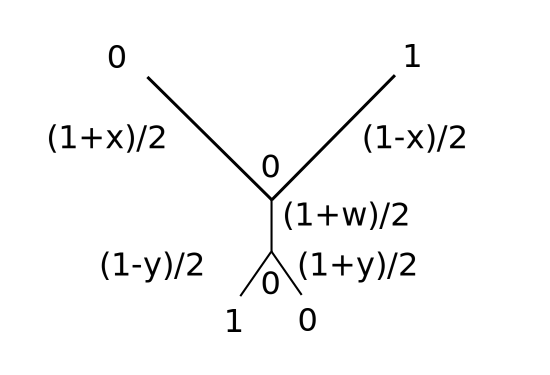
\includegraphics[width=.95\textwidth]{farris_like00}
\caption[short]{}
\end{subfigure}
\begin{subfigure}{.45\linewidth}
\centering
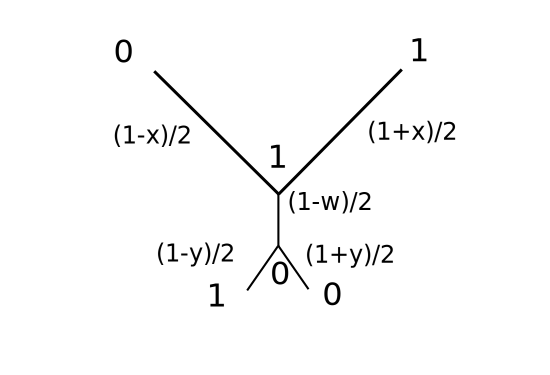
\includegraphics[width=.95\textwidth]{farris_like10}
\caption[short]{}
\end{subfigure}
\caption{
    Example likelihood computations on the InvFels tree $\tau_1$ for fidelities $t=\{x_1,y_1,x_2,y_2,w\}$.
    Edges labeled by the probability of substitution along that edge.
    In (a), we compute the product to obtain $\Pr(\ancestralSplitRV=\emptyset\mid \siteSplitRV=\{2,3\},\tau_1,t) = (1+x_1)(1-x_2)(1+y_1)(1-y_2)(1+w)/32$.
    In (b), the same process yields $\Pr(\ancestralSplitRV=\{1\}\mid \siteSplitRV=\{2,3\},\tau_1,t) = (1+x_1)(1-x_2)(1+y_1)(1-y_2)(1-w)/32$.
}
\label{fig:example_likelihoods}
\end{figure}

\begin{table}
\centering
\begin{tabular}{|l|ll|}
\hline
$\siteSplit_j$ & $\ancestralSplit_k$ & $32\cdot\Pr(\ancestralSplitRV=\ancestralSplit_k \mid \siteSplitRV=\siteSplit_j, \tau_1, t)$\\
\hline
$\emptyset$&$\emptyset$&$(1+x_1)(1+y_1)(1+x_2)(1+y_2)(1+w)$\\
&$\{1\}^*$&$(1-x_1)(1+y_1)(1-x_2)(1+y_2)(1-w)$             \\
&$\{2\}^*$&$(1+x_1)(1-y_1)(1+x_2)(1-y_2)(1-w)$             \\
&$\{1,2\}^*$&$(1-x_1)(1-y_1)(1-x_2)(1-y_2)(1+w)$           \\

$\{1\}$    &$\emptyset$&$(1-x_1)(1+y_1)(1+x_2)(1+y_2)(1+w)$\\
&$\{1\}$&$(1+x_1)(1+y_1)(1-x_2)(1+y_2)(1-w)$               \\
&$\{2\}^*$&$(1-x_1)(1-y_1)(1+x_2)(1-y_2)(1-w)$             \\
&$\{1,2\}$&$(1+x_1)(1-y_1)(1-x_2)(1-y_2)(1+w)$             \\

$\{2\}$    &$\emptyset$&$(1+x_1)(1-y_1)(1+x_2)(1+y_2)(1+w)$\\
&$\{1\}^*$&$(1-x_1)(1-y_1)(1-x_2)(1+y_2)(1-w)$             \\
&$\{2\}$&$(1+x_1)(1+y_1)(1+x_2)(1-y_2)(1-w)$               \\
&$\{1,2\}$&$(1-x_1)(1+y_1)(1-x_2)(1-y_2)(1+w)$             \\

$\{3\}$    &$\emptyset$&$(1+x_1)(1+y_1)(1-x_2)(1+y_2)(1+w)$\\
&$\{1\}$&$(1-x_1)(1+y_1)(1+x_2)(1+y_2)(1-w)$               \\
&$\{2\}^*$&$(1+x_1)(1-y_1)(1-x_2)(1-y_2)(1-w)$             \\
&$\{1,2\}$&$(1-x_1)(1-y_1)(1+x_2)(1-y_2)(1+w)$             \\

$\{1,2,3\}$&$\emptyset$&$(1-x_1)(1-y_1)(1-x_2)(1+y_2)(1+w)$\\
&$\{1\}$&$(1+x_1)(1-y_1)(1+x_2)(1+y_2)(1-w)$               \\
&$\{2\}^*$&$(1-x_1)(1+y_1)(1-x_2)(1-y_2)(1-w)$             \\
&$\{1,2\}$&$(1+x_1)(1+y_1)(1+x_2)(1-y_2)(1+w)$             \\

$\{1,2\}$  &$\emptyset$&$(1-x_1)(1-y_1)(1+x_2)(1+y_2)(1+w)$\\
&$\{1\}$&$(1+x_1)(1-y_1)(1-x_2)(1+y_2)(1-w)$               \\
&$\{2\}$&$(1-x_1)(1+y_1)(1+x_2)(1-y_2)(1-w)$               \\
&$\{1,2\}$&$(1+x_1)(1+y_1)(1-x_2)(1-y_2)(1+w)$             \\

$\{2,3\}$  &$\emptyset$&$(1+x_1)(1-y_1)(1-x_2)(1+y_2)(1+w)$\\
&$\{1\}$&$(1-x_1)(1-y_1)(1+x_2)(1+y_2)(1-w)$               \\
&$\{2\}$&$(1+x_1)(1+y_1)(1-x_2)(1-y_2)(1-w)$               \\
&$\{1,2\}$&$(1-x_1)(1+y_1)(1+x_2)(1-y_2)(1+w)$             \\

$\{1,3\}$  &$\emptyset$&$(1-x_1)(1+y_1)(1-x_2)(1+y_2)(1+w)$\\
&$\{1\}$&$(1+x_1)(1+y_1)(1+x_2)(1+y_2)(1-w)$               \\
&$\{2\}^*$&$(1-x_1)(1-y_1)(1-x_2)(1-y_2)(1-w)$             \\
&$\{1,2\}$&$(1+x_1)(1-y_1)(1+x_2)(1-y_2)(1+w)$             \\
\hline
\end{tabular}
\caption{
32 times conditional likelihood values for all site splits $\siteSplit_j$ and ancestral state splits $\ancestralSplit_k$ of the InvFels tree $\tau_1$.
Ancestral states with $^*$ are never maximal provided parameters are in $(0,1]$.
By combinations of $\ancestralSplit_k$, there are $3^5\cdot 4^2=3,888$ possible forms for the conditional likelihood.
}
\label{tab:farris_likelihoods}
\end{table}

%TODO: the caption of this overlaps with the page number---will this be a problem or will MBE handle it?
%EM There is a latex package for that, which I tried out and then removed for some reason. It's no bigs.

\subsection*{Convergence of branch parameters}

%das: @EM I think this is actually the same Wald reference that Felsenstein tried to use.
%It works here for a fixed topology, and didn't work for him or your reference because I think the upper-semicontinuous condition doesn't hold for trees in general.
%Also I don't think the compactness condition holds---tree space isn't compact is it?
%However we now have a potential snag in that we are doing what Yang (1994) in his intro says is bad, i.e., doing ML for fixed, separate topologies and comparing them.
%We still have the behavior in the plots and the proofs, since they all assumed a fixed topology, and I think everything's fine with the arguments about Fels vs InvFels, but maybe you can let me know what you think?
For a fixed $\tau$, we show that $\hat{t}_\nCols \rightarrow \hat{t}$ for
\[
\hat{t}_\nCols = \arg\max_{t\in\mathcal{T}} \ \frac{1}{n}\log L_\nCols'(\tau, t; \fullAlignment)
\]
and
\[
\hat{t} = \arg\max_{t\in\mathcal{T}} \ \ell_{\tau^*,t^*}(\tau, t; \boldsymbol\xi).
\]
%EM perhaps a section reference for this big book?
Using the notation in \citet{van1998asymptotic}, we let
\[
m_t(\alignmentColumn) = \sum_{j=1}^\nSiteSplits 1\{\patternToSplit(\alignmentColumn)=\siteSplit_j\} \cdot [\log \Pr(\siteSplitRV=\siteSplit_j \mid \tau, t) + \log \Pr(\ancestralSplitRV=\xi_j \mid \siteSplitRV=\siteSplit_j , \tau, t)]
\]
so that
\[
\frac{1}{n}\log L_\nCols'(\tau, t; \fullAlignment) = \frac{1}{n} \sum_{i=1}^\nCols m_t(\alignmentColumn_i)
\]
and
\[
\ell_{\tau^*,t^*}(\tau, t; \boldsymbol\xi) = E[m_t].
\]
To show $\hat{t}_\nCols \rightarrow \hat{t}$, we use Wald's consistency proof \citep[p. 48, Theorem 5.14 of ][]{van1998asymptotic}, which requires four conditions.
The first is that $\mathcal{T}$ is compact, which is obviously true.
The second is that
\[
E\left[\sup_{t\in\mathcal{T}} m_t\right] < \infty,
\]
and, since $m_t(\alignmentColumn)$ is nonpositive for all $t$ and $\alignmentColumn$, this property holds.
The remaining conditions are on the maps
\[
\alignmentColumn \mapsto \sup_t m_t(\alignmentColumn)
\]
and
\[
t \mapsto m_t(\alignmentColumn).
\]
We need the first map to be measurable, which is evident since the domain $\alphabet^\nSiteRows$ of the mapping is a finite set, and so all subsets of the domain are also finite and thus measurable.
Finally, we must have the the second mapping be upper-semicontinuous for almost all $\alignmentColumn$.
For a fixed ancestral state split $t \mapsto m_t(\alignmentColumn)$ is continuous for all $\alignmentColumn$.
If we move about in $\mathcal{T}$, a different ancestral state split becomes more likely, though when we maximize over ancestral state splits we obtain a continuous function since the maximum over continuous functions is also continuous.
This ensures the upper-semicontinuous property of this mapping, and shows $\hat{t}_\nCols \rightarrow \hat{t}$, allowing our consistency results to be proved using $\ell_{\tau^*,t^*}(\tau, t; \boldsymbol\xi)$.

\subsection*{Properties of the joint objective function}

Consider the InvFels tree $\tau_1$ with arbitrary fidelities, i.e., $t=\{x_1,y_1,x_2,y_2,w\}$.
Next we show that the likelihood $\ell_{\tau_1,t^*}(\tau_1, t; \boldsymbol\xi)$ remains unchanged if $x_1$ and $x_2$ are exchanged or if $y_1$ and $y_2$ are.
Using the Hadamard transform, we calculate the generating probabilities on the InvFels tree.
For site split $\emptyset$,
\begin{align*}
    \Pr(\siteSplitRV=\emptyset\mid \tau_1, t) & = \frac{1}{8} (1 + x_1x_2 +  y_1y_2 +  x_1y_1w + x_1y_2w + y_1x_2w + x_2y_2w + x_1y_1x_2y_2) \\
                                              & = \frac{1}{8} (1 + x_1x_2 +  y_1y_2 +  w[x_1y_1 + x_1y_2 + y_1x_2 + x_2y_2] + x_1y_1x_2y_2) \\
                                              & = \frac{1}{8} (1 + x_1x_2 +  y_1y_2 +  w[x_1 + x_2][y_1 + y_2] + x_1y_1x_2y_2),
\end{align*}
and this probability is unchanged when $x_1$ is exchanged with $x_2$ and $y_1$ is exchanged with $y_2$.

All other generating probabilities differ only in the signs of each term (see Table~\ref{tab:gen-sitepatprob}).
For example, for site split $\{1\}$ we have
\begin{align*}
    \Pr(\siteSplitRV=\{1\}\mid \tau_1, t) & = \frac{1}{8} (1 - x_1x_2 +  y_1y_2 +  w[-x_1 + x_2][y_1 + y_2] - x_1y_1x_2y_2)
\end{align*}
and for site split $\{3\}$ we have
\begin{align*}
    \Pr(\siteSplitRV=\{3\}\mid \tau_1, t) & = \frac{1}{8} (1 - x_1x_2 +  y_1y_2 +  w[x_1 - x_2][y_1 + y_2] - x_1y_1x_2y_2)
\end{align*}
meaning if we exchange the values of $x_1$ and $x_2$ then these probabilities swap values.
We show that for site splits $\{1\}$ and $\{3\}$, exchanging $x_1$ and $x_2$ also swaps the values of the conditional likelihood terms (Table~\ref{tab:farris_likelihoods}).
Indeed, the corresponding possibilities for the conditional likelihood values are
\begin{align*}
    \Pr(\ancestralSplitRV=\emptyset \mid \siteSplitRV=\{1\}, \tau_1, t) &= \frac{1}{32}(1-x_1)(1+x_2)(1+w)(1+y_1)(1+y_2); \\
    \Pr(\ancestralSplitRV=\{1\} \mid \siteSplitRV=\{1\}, \tau_1, t) &= \frac{1}{32}(1+x_1)(1-x_2)(1-w)(1+y_1)(1+y_2); \\
    \Pr(\ancestralSplitRV=\{2\} \mid \siteSplitRV=\{1\}, \tau_1, t) &= \frac{1}{32}(1-x_1)(1+x_2)(1-w)(1-y_1)(1-y_2); \\
    \Pr(\ancestralSplitRV=\{1,2\} \mid \siteSplitRV=\{1\}, \tau_1, t) &= \frac{1}{32}(1+x_1)(1-x_2)(1+w)(1-y_1)(1-y_2);
\end{align*}
for site split $\{1\}$ and
\begin{align*}
        \Pr(\ancestralSplitRV=\emptyset \mid \siteSplitRV=\{3\}, \tau_1, t) &= \frac{1}{32}(1+x_1)(1-x_2)(1+w)(1+y_1)(1+y_2); \\
    \Pr(\ancestralSplitRV=\{1\} \mid \siteSplitRV=\{3\}, \tau_1, t) &= \frac{1}{32}(1-x_1)(1+x_2)(1-w)(1+y_1)(1+y_2); \\
    \Pr(\ancestralSplitRV=\{2\} \mid \siteSplitRV=\{3\}, \tau_1, t) &= \frac{1}{32}(1+x_1)(1-x_2)(1-w)(1-y_1)(1-y_2); \\
    \Pr(\ancestralSplitRV=\{1,2\} \mid \siteSplitRV=\{3\}, \tau_1, t) &= \frac{1}{32}(1-x_1)(1+x_2)(1+w)(1-y_1)(1-y_2);
\end{align*}
for site split $\{3\}$, which shows the likelihood remains unchanged if $x_1$ and $x_2$ are swapped.
The same can be done for the splits $\{2\}$ and $\{1,2,3\}$ by exchanging $y_1$ and $y_2$
%EM does this one need a different explanation now?
as well as $\{1,2\}$ and $\{2,3\}$ by exchanging both $x_1$ with $x_2$ and $y_1$ with $y_2$.
The split $\{1,3\}$ is unchanged by exchanging $x_1$ with $x_2$ and $y_1$ with $y_2$.
Exchanging $x_1$ and $x_2$ also does not change the value of the log-likelihood $\ell_{\tau_1,t^*}(\tau_1, t; \boldsymbol\xi)$.

Thus, we can reduce the number of candidate likelihoods we need to search by, without loss of generality, assuming $x_2 \ge x_1$.
An analogous statement holds for $y_2 \ge y_1$, with these conditional likelihoods given in Table~\ref{tab:likelihoods} after maximizing over ancestral state splits.

\begin{table}
\centering
\begin{tabular}{|lll|l|}
\hline
$\siteSplit_j$ & $\ancestralSplitPartition_j(\tau_1, t)$ & $\xi_j$ & $32\cdot\Pr(\ancestralSplitRV=\xi_j \mid \siteSplitRV=\siteSplit_j,\tau_1,t)$\\
\hline
$\emptyset$&$\{\emptyset\}$&$\emptyset$&$(1+x_1)(1+y_1)(1+x_2)(1+y_2)(1+w)$\\

$\{1\}$    &$\{\emptyset\}$&$\emptyset$&$(1-x_1)(1+y_1)(1+x_2)(1+y_2)(1+w)$\\

$\{2\}$    &$\{\emptyset\}$&$\emptyset$&$(1+x_1)(1-y_1)(1+x_2)(1+y_2)(1+w)$\\

$\{3\}$    &$\{\emptyset,\{1\},\{1,2\}\}$&$\emptyset$&$(1+x_1)(1+y_1)(1-x_2)(1+y_2)(1+w)$\\
&&$\{1\}$&$(1-x_1)(1+y_1)(1+x_2)(1+y_2)(1-w)$\\
&&$\{1,2\}$&$(1-x_1)(1-y_1)(1+x_2)(1-y_2)(1+w)$\\

$\{1,2,3\}$&$\{\emptyset,\{1\},\{1,2\}\}$&$\emptyset$&$(1-x_1)(1-y_1)(1-x_2)(1+y_2)(1+w)$\\
&&$\{1\}$&$(1+x_1)(1-y_1)(1+x_2)(1+y_2)(1-w)$\\
&&$\{1,2\}$&$(1+x_1)(1+y_1)(1+x_2)(1-y_2)(1+w)$\\

$\{1,2\}$  &$\{\emptyset\}$&$\emptyset$&$(1-x_1)(1-y_1)(1+x_2)(1+y_2)(1+w)$\\

$\{2,3\}$  &$\{\emptyset,\{1\},\{1,2\}\}$&$\emptyset$&$(1+x_1)(1-y_1)(1-x_2)(1+y_2)(1+w)$\\
&&$\{1\}$&$(1-x_1)(1-y_1)(1+x_2)(1+y_2)(1-w)$\\
&&$\{1,2\}$&$(1-x_1)(1+y_1)(1+x_2)(1-y_2)(1+w)$\\

$\{1,3\}$  &$\{\emptyset,\{1\},\{1,2\}\}$&$\emptyset$&$(1-x_1)(1+y_1)(1-x_2)(1+y_2)(1+w)$\\
&&$\{1\}$&$(1+x_1)(1+y_1)(1+x_2)(1+y_2)(1-w)$\\
&&$\{1,2\}$&$(1+x_1)(1-y_1)(1+x_2)(1-y_2)(1+w)$\\
\hline
\end{tabular}
\caption{
32 times conditional likelihood values on the InvFels tree $\tau_1$.
Due to the symmetry of the likelihood, WLOG we assume $x_2 \ge x_1$ and $y_2 \ge y_1$ and maximize over ancestral state splits to reduce the number of possible functional forms to consider.
Likelihoods with multiple entries have maxima determined by unknown branch length parameters.
Because in 4 cases there are 3 possibilities for $\xi_j$, there are $3^4=81$ possible forms for the conditional likelihood.
}
\label{tab:likelihoods}
\end{table}

\subsection*{Theorems and proofs}

%where data is generated on the InvFels tree with two top branches of fidelity $x^*$ and all other branches of fidelity $y^*$ (Fig.~\ref{fig:farris-fels-top}).

We first prove intermediate results to show the main result.

\begin{lemma}
Let $\tau^*=\tau_1$, $t^*=\{x^*, y^*, x^*, y^*, y^*\}$, and $t=\{x_1, y_1, x_2, y_2, w\}$ with $x_1, y_1, x_2, y_2, w > 0$.
There exists a set of $0 < x^*, y^* < 1$ such that $\emptyset$ is the maximal ancestral state split for all site splits given $\tau=\tau_1$.
\label{lemma:ancestral-state}
\end{lemma}

\begin{proof}
Recall
\[
\ell_{\tau^*,t^*}(\tau, t; \boldsymbol\xi) = \shannonDivergence_{\tau^*,t^*}(\tau,t) + \ell^C_{\tau^*,t^*}(\tau, t; \boldsymbol\xi).
\]
We obtain
\[
\max_{t} \ \ell_{\tau^*,t^*}(\tau, t; \boldsymbol\xi) \le
    \shannonDivergence_{\tau^*,t^*}(\tau^*,t^*)
    + \ell^C_{\tau^*,t^*}(\tau, \tilde{t}; \boldsymbol\xi)
\]
as an upper bound for the joint maximum of \eqref{eq:log_likelihood_simplified} using Gibbs's inequality
\[
\shannonDivergence_{\tau^*,t^*}(\tau,t) \le \shannonDivergence_{\tau^*,t^*}(\tau^*,t^*)
\]
and
\[
\tilde{t} = \argmax_{t} \ \ell^C_{\tau^*,t^*}(\tau, t; \boldsymbol\xi).
\]
By straightforward calculus, the function $f(x)=a_1\log(1+x)+a_2\log(1-x)$ attains a maximum at $\hat{x} = (a_1-a_2)/(a_1+a_2)$, and so we have a closed form for each component of $\tilde{t}$.
Using this estimate, we have the lower bound
\[
\max_{t} \ \ell_{\tau^*,t^*}(\tau, t; \boldsymbol\xi) \ge
    \shannonDivergence_{\tau^*,t^*}(\tau,\tilde{t})
    + \ell^C_{\tau^*,t^*}(\tau, \tilde{t}; \boldsymbol\xi).
\]
Let $\boldsymbol\xi_0 = [\emptyset]_{j=1}^\nSiteSplits$ and
\[
\tilde{t}_{\boldsymbol\xi} = \argmax_{t} \ \ell^C_{\tau^*,t^*}(\tau_1, t; \boldsymbol\xi).
\]
Define
\[
C_0(x^*, y^*) :=
    \shannonDivergence_{\tau^*,t^*}(\tau_1,\tilde{t}_{\boldsymbol\xi_0})
    + \ell^C_{\tau^*,t^*}(\tau_1, \tilde{t}_{\boldsymbol\xi_0}; \boldsymbol\xi_0),
\]
i.e., the lower bound assuming $\emptyset$ is the maximal ancestral state split for all site splits and $\tau=\tau_1$.

We need only consider the remaining possibilities for choices of ancestral state splits in Table~\ref{tab:likelihoods} upon excluding cases of infinite branch lengths (i.e., any of $x_1,y_1,x_2,y_2,w$ equal to zero) and the redundant cases of $x_1 > x_2$ and $y_1 > y_2$, i.e.,
\[
C_1(x^*, y^*) :=
    \shannonDivergence_{\tau^*,t^*}(\tau^*,t^*)
    +  \max_{\boldsymbol\xi : \boldsymbol\xi \neq \boldsymbol\xi_0} \ \ell^C_{\tau^*,t^*}(\tau_1, \tilde{t}_{\boldsymbol\xi}; \boldsymbol\xi).
\]
We show in Fig.~\ref{fig:max-anc-state} the region where $C_0(x^*,y^*) > C_1(x^*,y^*)$.
\end{proof}

\begin{figure}
\centering
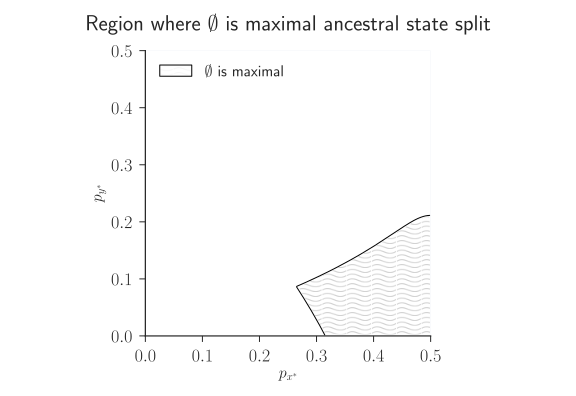
\includegraphics[width=.95\textwidth]{analytic-anc-state-inkscape}
\caption{
Region where $\emptyset$ is the maximal ancestral state split for each site split on the InvFels tree $\tau_1$.
}
\label{fig:max-anc-state}
\end{figure}

\begin{lemma}
Let $\tau^*=\tau_1$, $t^*=\{x^*, y^*, x^*, y^*, y^*\}$, and $t=\{x_1, y_1, x_2, y_2, w\}$ with $x_1, y_1, x_2, y_2, w > 0$.
For $0 < x^*, y^* < 1$ and $\boldsymbol\xi_0 = [\emptyset]_{j=1}^\nSiteSplits$, the solution $\hat{t} := \{\hat{x}_1,\hat{y}_1,\hat{x}_2,\hat{y}_2,\hat{w}\}$ given by
\[
\hat{t} = \arg\max_t \ell_{\tau^*, t^*}(\tau_1, t; \boldsymbol\xi_0)
\]
is subject to the constraints $\hat{x}_1,\hat{x}_2 \in (0, x^*]$, $\hat{y}_1 \in (0, y^*]$, and $\hat{y}_2,\hat{w} \in [y^*, 1]$.
\label{lemma:bounds}
\end{lemma}

\begin{proof}
We proceed by analyzing the gradients of each component of the likelihood function.
We first focus on the marginal log-likelihood
\[
\shannonDivergence_{\tau^*,t^*}(\tau_1,t) = \sum_{j=1}^\nSiteSplits \Pr(\siteSplitRV=\siteSplit_j \mid \tau^*, t^*) \cdot \log \Pr(\siteSplitRV=\siteSplit_j \mid \tau_1, t).
\]
By Gibbs' inequality, this function attains a unique maximum when
\[
\Pr(\siteSplitRV=\siteSplit_j \mid \tau_1, t) = \Pr(\siteSplitRV=\siteSplit_j \mid \tau^*, t^*)
\]
for all $j=1,\ldots,\nSiteSplits$ with $t^*=\{x^*,y^*,x^*,y^*,y^*\}$.
We show that this implies $t=t^*$.
Note that exchanging $x_1$ with $x_2$ and $y_1$ with $y_2$ does not affect the marginal log-likelihood, and, as it has a unique maximum, we have $x_1=x_2=x$ and $y_1=y_2=y$ at this maximum.
Referring to the top of Table~\ref{tab:gen-sitepatprob}, we set up simultaneous equations as follows.
The sum of generating probabilities for site splits $\{3\}$ and $\{1,2\}$ yields
\[
2-2(x^*)^2 = 2-2x^2
\]
and for $\{2\}$ and $\{1,2\}$ yields
\[
2-2(y^*)^2 = 2-2y^2.
\]
implying $x=x^*$ and $y=y^*$.
Setting these parameters to their optima, the difference of generating probabilities for site splits $\emptyset$ and $\{1,3\}$ yields
\[
8x^*(y^*)^2 = 8x^*y^*w
\]
implying $w=y^*$.
Thus the unique maximum is $\hat{t}=\{x^*,y^*,x^*,y^*,y^*\}$, and consequently
\[
\nabla_t \shannonDivergence_{\tau^*,t^*}(\tau_1,t) \mid_{t=t^*} = 0.
\]
We now show that the gradient of the marginal log-likelihood is a decreasing function on $(0,1]$ in each variable.
The marginal log-likelihood as a function of $x_1$ is
\begin{align*}
\shannonDivergence(x_1) = \sum_j p_{\siteSplit_j} \log(c_{x_1,\siteSplit_j} + a_{x_1,\siteSplit_j}x_1) - \log 8
\end{align*}
where $c_{x_1,\siteSplit_j}$ and $a_{x_1,\siteSplit_j}$ are functions of $y_1,x_2,y_2,$ and $w$.
For example, reading from Table~\ref{tab:gen-sitepatprob},
\[
c_{x_1,\emptyset} = 1+y_1y_2+wx_2y_1+wx_2y_2
\]
and
\[
a_{x_1,\emptyset} = x_2+wy_1+wy_2+x_2y_1y_2
\]
with similar definitions for the remaining site splits.
By the assumption of $0 < x^*, y^* < 1$, we have $p_{\siteSplit_j} > 0$ for $j=1,\ldots,\nSiteSplits$, therefore we assume $c_{x_1,\siteSplit_j} + a_{x_1,\siteSplit_j}x_1 \neq 0$ for all $j$ otherwise we obtain a zero value for our likelihood, i.e., $\shannonDivergence\rightarrow -\infty$.
In other words, we make the assumption that $x_1,y_1,x_2 < 1$, precluding all cases where $c_{x_1,\siteSplit_j} + a_{x_1,\siteSplit_j}x_1 = 0$ for some $j$.
This assumption is reasonable as the likelihood is never maximized at these values where $c_{x_1,\siteSplit_j} + a_{x_1,\siteSplit_j}x_1 = 0$.
Moreover, we have
\[
\Pr(\siteSplitRV=\siteSplit_j \mid \tau_1,\{x_1,y_1,x_2,y_2,w\}) = \frac{1}{8} (c_{x_1,\siteSplit_j} + a_{x_1,\siteSplit_j}x_1),
\]
which, being a probability, is greater than or equal to zero.
Consider the derivative with respect to $x_1$
\begin{align*}
\frac{d}{dx_1} \shannonDivergence(x_1) = \sum_j \frac{p_{\siteSplit_j}a_{x_1,\siteSplit_j}}{c_{x_1,\siteSplit_j} + a_{x_1,\siteSplit_j}x_1}
\end{align*}
and focus on the $j$th term in the summation
\[
f_j(x_1) := \frac{p_{\siteSplit_j}a_{x_1,\siteSplit_j}}{c_{x_1,\siteSplit_j} + a_{x_1,\siteSplit_j}x_1}.
\]
%das: gah, had to roll back this line and add some stuff above since there are cases where some probabilities are 0. Maybe I'm being too careful? I don't think it's an issue, just an edge case that could induce wonkiness, so I included an assumption.
Regardless of $a_{x_1,\siteSplit_j} \lessgtr 0$, $f_j$ is a decreasing function of $x_1$ as $c_{x_1,\siteSplit_j} + a_{x_1,\siteSplit_j}x_1 > 0$.
The remaining variables follow similar arguments.

\begin{table}
\centering
\begin{tabular}{|lll|l|}
\hline
$\siteSplit_j$ & $\ancestralSplitPartition_j(\tau_1, t)$ & $\xi_j$ & $32\cdot\Pr(\ancestralSplitRV=\xi_j \mid \siteSplitRV=\siteSplit_j,\tau_1,t)$\\
\hline
$\emptyset$&$\{\emptyset\}$&$\emptyset$&$(1+x_1)(1+y_1)(1+x_2)(1+y_2)(1+w)$\\
$\{1\}$    &$\{\emptyset\}$&$\emptyset$&$(1-x_1)(1+y_1)(1+x_2)(1+y_2)(1+w)$\\
$\{2\}$    &$\{\emptyset\}$&$\emptyset$&$(1+x_1)(1-y_1)(1+x_2)(1+y_2)(1+w)$\\
$\{3\}$    &$\{\emptyset,\{1\},\{1,2\}\}$&$\emptyset$&$(1+x_1)(1+y_1)(1-x_2)(1+y_2)(1+w)$\\
$\{1,2,3\}$&$\{\emptyset,\{1\},\{1,2\}\}$&$\emptyset$&$(1-x_1)(1-y_1)(1-x_2)(1+y_2)(1+w)$\\
$\{1,2\}$  &$\{\emptyset\}$&$\emptyset$&$(1-x_1)(1-y_1)(1+x_2)(1+y_2)(1+w)$\\
$\{2,3\}$  &$\{\emptyset,\{1\},\{1,2\}\}$&$\emptyset$&$(1+x_1)(1-y_1)(1-x_2)(1+y_2)(1+w)$\\
$\{1,3\}$  &$\{\emptyset,\{1\},\{1,2\}\}$&$\emptyset$&$(1-x_1)(1+y_1)(1-x_2)(1+y_2)(1+w)$\\
\hline
\end{tabular}
\caption{
32 times the maximal conditional likelihood values on the InvFels tree $\tau_1$ assuming $\emptyset$ is the most likely ancestral state split for each site split.
}
\label{tab:likelihoods-restricted}
\end{table}

We now focus on the conditional log-likelihood.
Assume $\emptyset$ is the most likely ancestral state split for all site splits.
In this case, the conditional log-likelihood has no ambiguity, and has terms given as the log of those in Table~\ref{tab:likelihoods-restricted}.
We focus on the derivative with respect to $x_1$, aggregating all terms involving $x_2,y_1,y_2,$ and $w$ into a constant term.
The conditional log-likelihood
\[
\ell^C_{\tau^*,t^*}(\tau_1, t; \boldsymbol\xi_0) = \sum_{j=1}^\nSiteSplits \Pr(\siteSplitRV=\siteSplit_j \mid \tau^*, t^*)\cdot\log \Pr(\ancestralSplitRV=\emptyset \mid \siteSplitRV = \siteSplit_j, \tau_1, t),
\]
using Tables~\ref{tab:gen-sitepatprob} and~\ref{tab:likelihoods-restricted}, is
\begin{align*}
\ell^C(x_1; \boldsymbol\xi_0) &= \left(\frac{1}{2}+\frac{1}{2}x^*(y^*)^2\right)\log(1+x_1) + \left(\frac{1}{2}-\frac{1}{2}x^*(y^*)^2\right)\log(1-x_1)\\
&\qquad + \left(\frac{1}{2}+\frac{1}{2}(y^*)^2\right)\log(1+y_1) + \left(\frac{1}{2}-\frac{1}{2}(y^*)^2\right)\log(1-y_1)\\
&\qquad + \left(\frac{1}{2}+\frac{1}{2}x^*(y^*)^2\right)\log(1+x_2) + \left(\frac{1}{2}-\frac{1}{2}x^*(y^*)^2\right)\log(1-x_2)\\
&\qquad + \log(1+y_2) + \log(1+w) - \log 32\\
&:= \left(\frac{1}{2}+\frac{1}{2}x^*(y^*)^2\right)\log(1+x_1) + \left(\frac{1}{2}-\frac{1}{2}x^*(y^*)^2\right)\log(1-x_1)\\
&\qquad + C_{x_1}(x_2,y_1,y_2,w).
\end{align*}
where $C_{x_1}$ is a function of $y_1,x_2,y_2,$ and $w$.
The derivative with respect to $x_1$ is
\[
\frac{d}{dx_1} \ell^C(x_1; \boldsymbol\xi_0) = \frac{-x_1+x^*(y^*)^2}{1-x_1^2}
\]
which is negative for all $x_1 \ge x^*$.
This same process applied to the remaining variables shows the gradient of the full likelihood is negative for $x_1,x_2 \ge x^*$ and $y_1 \ge y^*$ and positive for $y_2,w \ge y^*$, yielding the constraints
\[
\hat{x}_1,\hat{x}_2 \in (0, x^*], \ \hat{y}_1 \in (0, y^*], \text{and}\ \hat{y}_2,\hat{w} \in [y^*, 1].
\]
\end{proof}

Since $x^*, y^* < 1$, the assumption that $x_1,y_1,x_2 < 1$ does not contradict with the statement of Lemma~\ref{lemma:bounds}.
We now prove the main result.

\topoInconsist*

\begin{proof}
We proceed as in the previous proof by simplifying the constants in the log-likelihood.
We analyze the derivative with respect to $w$, so we absorb all terms of only $x_1,y_1,x_2,$ and $y_2$ into a constant that disappears upon taking the derivative.
The objective function is
\begin{align*}
\ell(w; \boldsymbol\xi_0) = \left(\sum_j p_{\siteSplit_j} \log(c_{w,\siteSplit_j} + a_{w,\siteSplit_j}w)\right) + \log(1+w) + C_w(x_1,y_1,x_2,y_2)
\end{align*}
where $c_{w,\siteSplit_j},a_{w,\siteSplit_j}$ and $C_w$ are functions of $x_1,y_1,x_2,$ and $y_2$.
Using the middle panel of Table~\ref{tab:gen-sitepatprob}, we obtain
\[
c_{w,\emptyset} = 1+x_1x_2+y_1y_2+x_1y_1x_2y_2 = (1+x_1x_2)(1+y_1y_2)
\]
and
\[
a_{w,\emptyset} = x_1y_1+x_1y_2+x_2y_1+x_2y_2 = (x_1+x_2)(y_1+y_2)
\]
with similar definitions for the remaining site splits.
We make a further simplification on our way to computing bounds on the likelihood.
Let
\begin{align*}
\ell(w; \boldsymbol\xi_0) &= \left(\sum_j p_{\siteSplit_j} \log(c_{w,\siteSplit_j} + a_{w,\siteSplit_j}w)\right) + \log(1+w) + C_w(x_1,y_1,x_2,y_2) \\
        &= \left(\sum_j p_{\siteSplit_j} \log(c_{w,\siteSplit_j} + a_{w,\siteSplit_j}w) - p_{\siteSplit_j} \log(c_{w,\siteSplit_j})\right) + \log(1+w) \\
        &\qquad + \left(C_w(x_1,y_1,x_2,y_2) + \sum_j p_{\siteSplit_j} \log(c_{w,\siteSplit_j})\right) \\
        &=: \left(\sum_j p_{\siteSplit_j} \log(1 + b_{w,\siteSplit_j}w)\right) + \log(1+w) + C^*_w(x_1,y_1,x_2,y_2)
\end{align*}
where
\[
b_{\emptyset} := \frac{a_{w,\emptyset}}{c_{w,\emptyset}} = \frac{(x_1+x_2)(y_1+y_2)}{(1+x_1x_2)(1+y_1y_2)}
\]
with similar definitions for the remaining site splits.
The derivative with respect to $w$ of this function is
\begin{align*}
\ell'(w) := \frac{d}{dw} \ell(w; \boldsymbol\xi_0) =  \left(\sum_j \frac{p_{\siteSplit_j}b_{\siteSplit_j}}{1 + b_{\siteSplit_j}w}\right) + \frac{1}{1+w}.
\end{align*}
Using the fact that $b_{\emptyset} = -b_{13}$, $b_{1} = -b_{3}$, $b_{2} = -b_{123}$, and $b_{12} = -b_{23}$ in addition to $p_{1} = p_{3}$, $p_{2} = p_{123}$, and $p_{12} = p_{23}$, we simplify the derivative as
\begin{align*}
\ell'(w) &=  \frac{p_{\emptyset}b_{\emptyset}}{1 + b_{\emptyset}w} - \frac{p_{13}b_{\emptyset}}{1 - b_{\emptyset}w} + \frac{p_{2}b_{2}}{1 + b_{2}w} - \frac{p_{2}b_{2}}{1 - b_{2}w} \\
         &\qquad + \frac{p_{1}b_{1}}{1 + b_{1}w} - \frac{p_{1}b_{1}}{1 - b_{1}w} + \frac{p_{12}b_{12}}{1 + b_{12}w} - \frac{p_{12}b_{12}}{1 - b_{12}w} + \frac{1}{1+w}.\\
\end{align*}
Using the bounds on $\hat{x}_1,\hat{y}_1,\hat{x}_2$, and $\hat{y}_2$ from Lemma~\ref{lemma:bounds} and our assumption of $y_2 \ge y_1 > 0$ and $x_2 \ge x_1 > 0$, we have
\[
0 < b_{\emptyset} \le \frac{2x^*}{1+(x^*)^2} =: b_{\emptyset}^U,
\]
%das: The lower bound for b_{\emptyset} is strict because we assume x_1,...,w > 0, but for the other three they aren't strict since x_1 could equal x_2 and/or y_1 could equal y_2. This doesn't affect any later results, though, b/c b -> 0 just makes that term drop out.
\[
0 \le b_{2} \le \frac{2x^*}{1+(x^*)^2}\cdot\frac{1}{1-y^*} =: b_{2}^U,
\]
\[
0 \le b_{1} \le \frac{x^*}{1-(x^*)^2} =: b_{1}^U,
\]
\[
0 \le b_{12} \le \frac{x^*}{1-(x^*)^2}\cdot\frac{1}{1-y^*} =: b_{12}^U,
\]
so that $\ell'(w)$ has lower bound
\[
\ell'_{L}(w) :=  -\frac{p_{13}}{1/b_{\emptyset}^U - w} - \frac{p_{2}}{1/b_{2}^U - w} - \frac{p_{1}}{1/b_{1}^U - w} - \frac{p_{12}}{1/b_{12}^U - w} + \frac{1}{1+w}.
\]
Each term in $\ell'_{L}(w)$ is of the form
\[
f(w) = \frac{p}{1/b + w} = \frac{p\cdot b}{1 + b\cdot w}
\]
with $0 \le p \le 1$.
Assume $b_{\emptyset}^U, b_{2}^U, b_{1}^U, b_{12}^U < 1$, so that $-1 < b < 1$.
Since $b > -1$ and $w\in(0,1]$, $1+b\cdot w > 0$ and, thus, each term in $\ell'_{L}(w)$ is a decreasing function in $w$.
Thus, if $\ell'_{L}(1) > 0$, since $\ell'_{L}(w)$ is decreasing on $(0,1]$ then $\ell'_{L}(w) > 0$ for all $w\in (0,1]$.
Since $\ell'(w) > \ell'_{L}(w)$ for $w\in(0,1]$, this implies $\ell'(w) > 0$, which further implies $\ell(w; \boldsymbol\xi_0)$ is increasing on the entire interval $(0,1]$, including at the boundary $w=1$, and $\hat{w} \equiv 1$.

%EM Topic sentence here please.
%das: made more explicit and introduced more gently
We now construct the conditions on $x^*$ and $y^*$ that are required for $\hat{w}\equiv 1$:
\[
C1-C3: b_{2}^U, b_{1}^U, b_{12}^U < 1,
\]
\[
C4: -\frac{p_{13}b_{\emptyset}^U}{1-b_{\emptyset}^U} - \frac{p_{2}b_{2}^U}{1-b_{2}^U} - \frac{p_{1}b_{1}^U}{1-b_{1}^U} - \frac{p_{12}b_{12}^U}{1-b_{12}^U} + \frac{1}{2} > 0.
\]
Conditions $C1-C3$ are needed so that $\ell'_{L}(w)$ is a decreasing function on $(0,1]$, while condition $C4$ is the one on $\ell'_{L}(1) > 0$, i.e., so that $\ell'(w)$ is positive on $(0,1]$.
The set of $x^*,y^*$ satisfying conditions $C1-C4$ as well as those for $\emptyset$ being the most likely ancestral state split is given in Fig.~\ref{fig:incons-analytic}, giving the region of generating parameters where $\hat{w}\equiv 1$.
\end{proof}

As the region in Fig.~\ref{fig:incons-analytic} gives the values of $x^*$ and $y^*$ where $\hat{w}$ is guaranteed to be one, we converge on a multifurcating topology in these cases.
It is easy to see that assuming $\emptyset$ for each maximal ancestral state split results in the same conditional log-likelihood for $\tau_1$ and $\tau_2$.
Moreover, if $w=1$, the internal branch becomes zero-length and the two topologies are indistinguishable.
Let $\mathcal{T}_0$ be such that, for $t^*=\{x^*,y^*,x^*,y^*,y^*\}$, $t^*\in\mathcal{T}_0$ corresponds to $x^*$ and $y^*$ falling in the shaded region in Fig.~\ref{fig:incons-analytic}.
We can see this results in the likelihood of both topologies being equal, i.e.,
\begin{align*}
\max_{t : t^*\in\mathcal{T}_0} & \ \ell_{\tau^*,t^*}(\tau_1, t; \boldsymbol\xi)\\
&= \max_{t: \boldsymbol\xi=\boldsymbol\xi_0, w=1, \tau=\tau_1} \ \sum_{j=1}^\nSiteSplits \Pr(\siteSplitRV=\siteSplit_j \mid \tau^*, t^*) \cdot \log \Pr(\siteSplitRV=\siteSplit_j \mid \tau, \{x_1,y_1,x_2,y_2,w\})\\
&\qquad + \Pr(\siteSplitRV=\siteSplit_j \mid \tau^*, t^*) \cdot \Pr(\ancestralSplitRV=\xi_j \mid \siteSplitRV=\siteSplit_j, \tau, \{x_1,y_1,x_2,y_2,w\})\\
&= \max_{t: \boldsymbol\xi=\boldsymbol\xi_0, w=1, \tau=\tau_2} \ \sum_{j=1}^\nSiteSplits \Pr(\siteSplitRV=\siteSplit_j \mid \tau^*, t^*) \cdot \log \Pr(\siteSplitRV=\siteSplit_j \mid \tau, \{x_1,y_1,x_2,y_2,w\}) \\
&\qquad + \Pr(\siteSplitRV=\siteSplit_j \mid \tau^*, t^*) \cdot \Pr(\ancestralSplitRV=\xi_j \mid \siteSplitRV=\siteSplit_j, \tau, \{x_1,y_1,x_2,y_2,w\}).
\end{align*}

%~~~
% Figures mentioned in main section of manuscript


\begin{figure}
\centering
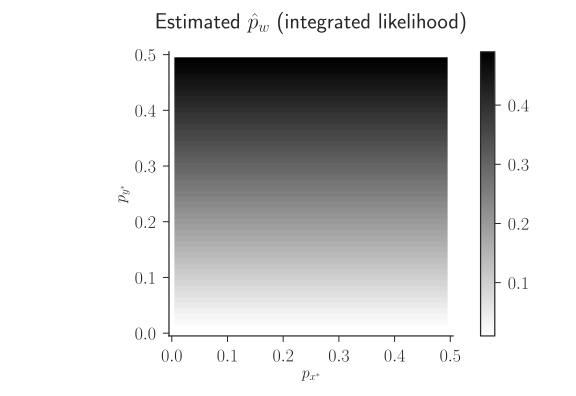
\includegraphics[width=\textwidth]{empirical-marginal}
\caption{
    Estimates for $\hat{p}_w$ when computing $(\hat{x}_1, \hat{y}_1, \hat{x}_2, \hat{y}_2, \hat{w})$ using L-BFGS-B optimizing the classical integrated likelihood \eqref{eq:marginal_likelihood} rather than a joint optimization procedure.
}
\label{fig:bl-general-marginal}
\end{figure}
%
%\begin{figure}
%\centering
%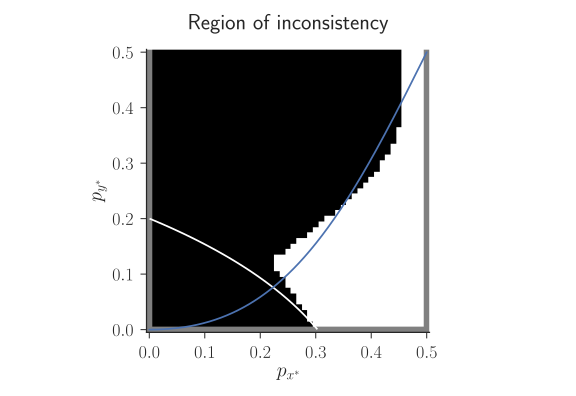
\includegraphics[width=.95\textwidth]{empirical-incons-intuition}
%\caption{
%Inconsistency in joint inference with intuitive curves.
%The white curve is our condition on the gradients.
%The blue curve is a condition on $x^*$ and $y^*$ such that $\emptyset$ is the most likely ancestral state.
%}
%\label{fig:empirical-incons-intuition}
%\end{figure}

